\section{Sensitivity Testing \& Robustness Analysis}
%书上写的是testing
%模型的分析，灵敏度分析和误差分析
%模型的检验（如果是建立模型前的检验可以在前面写，这里一般写对模型结果的检验）
%\subsection{Sensitivity Testing}

To clarify the parameter impact patterns of the Simulated Annealing algorithm in the emergency evacuation sweep model, we conduct the following sensitivity analysis.

\begin{figure}[htbp]
    \centering
    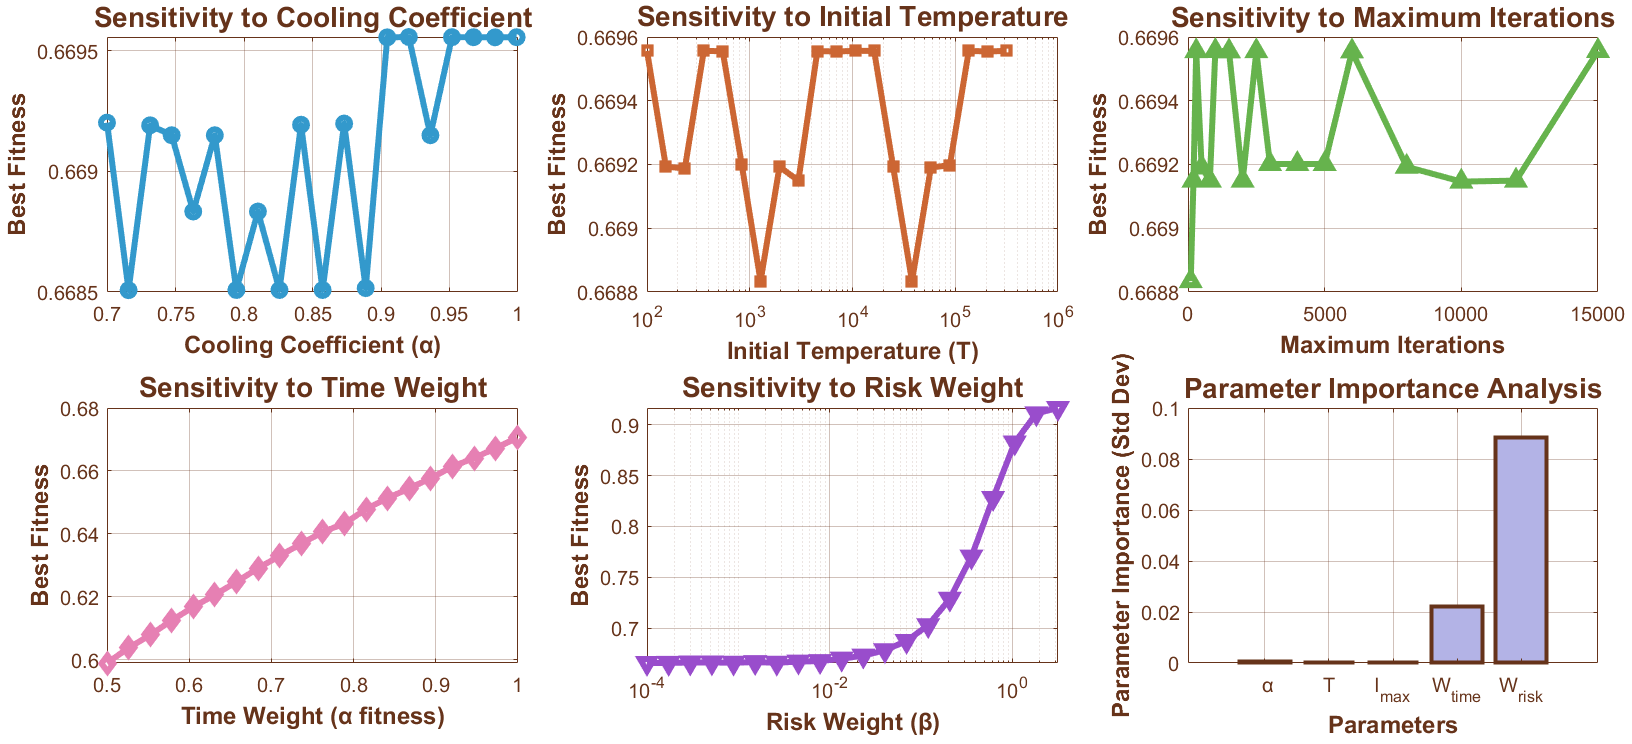
\includegraphics[width=1\linewidth]{fig/Simulated Annealing Parameter Sensitivity Analysis.png}
    \caption{Sensitivity Test to parameters in SA Algorithm}
    \label{fig:sens}
\end{figure}

Fig \ref{fig:sens} shows that the risk weight (\( W_{\text{risk}} \)) has the most significant impact on sweep efficiency, with a sharp rise in optimal fitness around \( 10^0 \) (strong positive effect). The time weight (\( W_{\text{time}} \)) presents a continuous positive effect, steadily improving path efficiency as its value increases. The initial temperature (\( T \approx 10^4 \)) and maximum number of iterations (\( I_{\text{max}} \)) are both related to whether the optimal solution (best fitness) can be achieved; however, due to the randomness of meta-heuristic algorithms, convergence to non-optimal solutions may occur, resulting in no regular changes in the curve over time. The cooling coefficient (\( \alpha \in [0.9,1] \)) has a weaker but stability-critical impact, with deviations beyond this range causing slower convergence. This analysis identifies core tuning parameters, providing a basis for model adaptation to different building layouts.



It provides key support for evacuation model optimization: first, it identifies \( W_{\text{risk}} \) and \( W_{\text{time}} \) as core decision parameters, whose impacts far exceed secondary variables like maximum iterations (\( I_{\text{max}} \)); second, it clarifies reasonable parameter ranges—for example, \( \alpha \) must be controlled between 0.9-1 to balance global search and convergence speed, reducing model uncertainty; third, it guides practical application decisions, allowing dynamic adjustment of \( W_{\text{risk}} \) based on building risk distribution and appropriate weight increase in complex buildings to ensure safety priority. The results verify the model’s robustness across multiple scenarios, enhancing solution feasibility.